\section{Choix}
\label{sec:choix}

\subsection{Distribution}
\label{subsec:distribution}

Le choix de la distribution s'est naturellement porté sur Debian, pour ses
nombreux avantages. En voici quelques exemples :
\begin{itemize}
\item Large communauté : grâce à cela, les erreurs et problèmes rencontrés ont
  souvent plusieurs solutions connues et éprouvées.

\item Plusieurs architectures et noyaux : Debian supporte la majorité des
  architectures de processeurs comme AMD, Armel, i386, MIPS, etc. Elle supporte
  aussi de nombreux noyaux tels que FreeBSD et GNU Hurd.

\item Sécurité : vu que la distribution est open-source, cela signifie que les
\textit{backdoors} sont presque inexistantes. De surcroît, lorsqu'une faille de
sécurité est détectée, celle-ci est rapidement corrigée par la communauté.

  En outre, Debian comprend de nombreux logiciels de sécurité tels que GPG (et
  PGP), SSH et autres.

\item Stabilité : les serveurs doivent avoir le plus grand temps d'accessibilité
($\approx$ 99.999\%). Sous Debian, il existe de nombreux exemples de machines
qui tournent sans arrêt pendant des années, mis à part lors de pannes ou de
mises à jour liées au matériel.

\item Système de paquets : grâce au système de paquets, les distributions Linux
  ont la possibilité d'installer de nombreux logiciels par une seule ligne de
  commande.
\end{itemize}

\begin{figure}[!h]
  \centering
  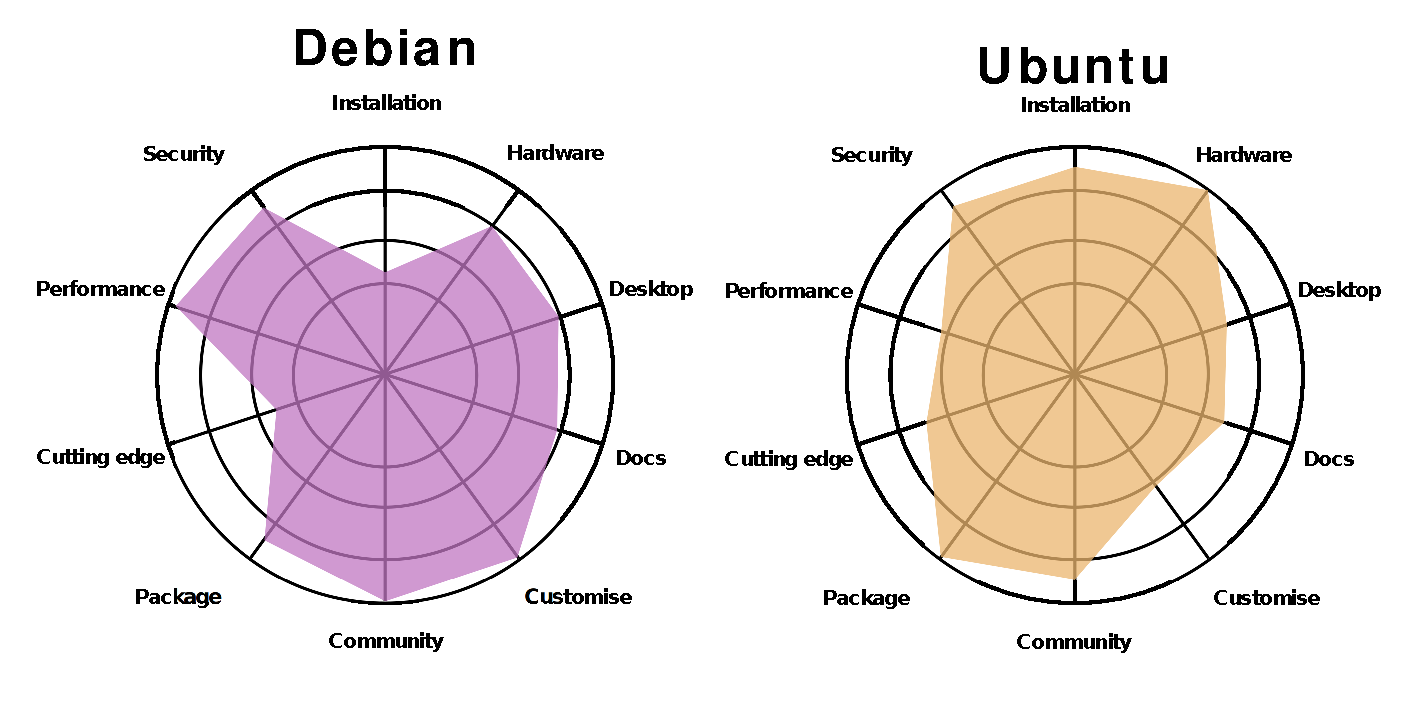
\includegraphics[width=0.75\textwidth]
  {textures/images/installation/DebianVsUbuntu.eps}
  \caption{Différences entre Debian et Ubuntu}
  \label{fig:diff-debian-ubuntu}
\end{figure}

\newpage

De même, la distribution Debian est plus professionnelle et celle-ci possède le
\textit{leadership} depuis des années.

\underline{Remarque :} depuis mai 2016, Ubuntu a les mêmes parts de marché que
Debian.

La distribution Ubuntu n'a pas été choisie pour les raisons suivantes :
\begin{itemize}
\item Dérivée de Debian : de ce fait, un administrateur sachant configurer un
serveur sous Debian pourra facilement s'adapter aux serveur sous Ubuntu.

\item Vise le grand public. Par conséquent, est beaucoup moins utilisé dans le
milieu professionnel.

\item Assez récente sur le marché du serveur.

\item Moins performante que Debian.
\end{itemize}

Concernant les autres distributions, CentOS est en baisse, mais reste au-dessus
de Red Hat et de Fedora qui sont en chute libre.

\begin{figure}[h]
  \centering
  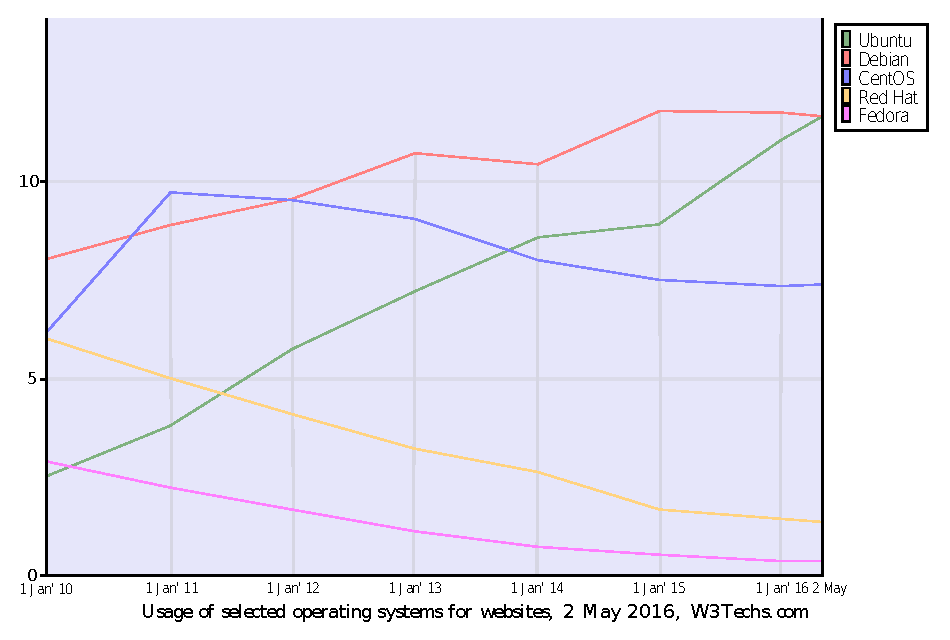
\includegraphics[width=0.8\textwidth]
  {textures/images/installation/distributions.eps}
  \caption{Parts de marché des distributions Linux}
\end{figure}

\newpage

\subsection{Langue}
\label{subsec:langue}

Pour le choix de la langue lors de l'installation, il a été préféré d'utiliser
l'anglais vu que la majorité des documentations et forums sont disponibles dans
cette langue. De plus, cela permet d'éviter une mauvaise traduction concernant
les nouvelles mises à jour et de toucher un large public le plus large possible.

\subsection{Noyau}
\label{subsec:noyau}

Un noyau (monolithique\footnote{Les fonctions du système et pilotes sont
regroupés dans le kernel space généré à la compilation.}) modulaire a été
choisi afin de gérer les modules. En effet, celui-ci facilite l'ajout et la
suppression de modules à chaud. Ces modules, pas toujours indispensables,
peuvent être la source de failles et de bugs.

\subsection{Partitionnement}
\label{subsec:partitionnement}

Le partionnement du disque a été réalisé avec une partition racine,
\textit{/boot}, et un groupe de volume LVM nommé \textit{VolGroup}. De surcroit,
deux disques de 10 Go en RAID 1 ont été utilisés.

\begin{center}
  \begin{table}[h]
    \begin{tabularx}{\linewidth}{|C|C|C|C|}
      \hline
      Label & Type & Taille (Mo) & Format \\
      \hline
      \hline
      /boot & primary & 512 & ext4 \\
      \hline
      VolGroup & logical & 20958 & lvm \\
      \hline
    \end{tabularx}

    \vskip .5cm

    \begin{tabularx}{\linewidth}{|C|C|C|C|}
      \hline
      LVsrv (/srv) & lvm & 6144 & ext4 \\
      \hline
      LVswap (/swap) & lvm & 4096 & swap \\
      \hline
      LVhome (/home) & lvm & 2048 & ext4 \\
      \hline
      LVroot (/root) & lvm & 2048 & ext4 \\
      \hline
      LVusr (/usr) & lvm & 2048 & ext4 \\
      \hline
      LVopt (/opt) & lvm & 2048 & ext4 \\
      \hline
      LVvar (/var) & lvm & 1024 & ext4 \\
      \hline
      LVtmp (/tmp) & lvm & 1024 & ext4 \\
      \hline
    \end{tabularx}
    \caption{Tableau du partitionnement \emph{(avec LVM)}}
    \label{tab:tableau-partitionnement}
  \end{table}
\end{center}

\subsection{Sauvegardes}
\label{subsec:sauvegardes}

Dans le milieu de l'entreprise, deux types de sauvegarde sont principalement
utilisés : incrémentielle\footnote{Sauvegarde exclusivement les données
modifiées ou ajoutées depuis la précédente sauvegarde.} et différentielle
\footnote{Sauvegarde les données modifiées ou ajoutées en référence à la
dernière sauvegarde complète.}.

Afin de trouver un compromis, ces deux types de sauvegardes ont été utilisés :

\begin{enumerate}
\item différentielle : afin de restaurer les données plus rapidement par rapport
  à la sauvegarde incrémentielle ;

\item incrémentielle : pour une rapidité de sauvegarde et un stockage en mémoire
plus économe que la sauvegarde différentielle.
\end{enumerate}

Dans le but d'éviter de perturber l'accès au serveur, tous les jours à deux heures du matin, une
sauvegarde incrémentielle est lancée à l'aide d'un
\emph{cron}\footnote{Gestionnaire des tâches sous Linux devant être exécutées à
un moment précis.}, dans le but d'enregistrer les données modifiées et créées en
cette journée.

\begin{lstlisting}[language=bash]
crontab -e 0 2 * * * /usr/bin/backup-make.sh -i
\end{lstlisting}

Quant à la sauvegarde différentielle, celle-ci s'opère uniquement le dimanche à
2 heures du matin. Le dimanche étant un jour de congé pour la majorité du monde,
ce qui aura un impact mineur sur les performances du serveur.

\begin{lstlisting}[language=bash]
crontab -e 0 2 * * 0 /usr/bin/backup-make.sh -d
\end{lstlisting}

\underline{Remarque :} à défaut d'utiliser \textit{fcron} n'étant plus
disponible sur Debian, le serveur doit être alimenté à l'heure de l'exécution du
\textit{cron}. Néanmoins, cela ne pose pas de difficultés, vu que le rôle du
serveur est de fournir une disponibilité permanente.

\newpage
\subsection{Sécurité des mots de passe}
\label{subsec:securite-mdps}

Afin de sécuriser l'accès au serveur, le mot de passe de l'administrateur est
\og \textbf{4c,4cs,1lM\&6lm.} \fg. \\
Il a une longueur de 15 caractères et est composé de 4 chiffres, 4 caractères
spéciaux, 1 lettre majuscule et 6 lettres minuscules. \\

Dans le meilleur des cas, tous les mots de passes seraient semblables, dans leur
force, mais différents dans leur forme. \\
Afin de nous simplifier la tâche lors de la présentation, nous avons décidé que
tous les mots de passe, \emph{autres que celui de l'administrateur}, seraient
\og \textbf{test} \fg. \\

Les différents logins sont donc :
\begin{itemize}

    \item administrateur : root - \textbf{4c,4cs,1lM\&6lm.};
    \item utilisateur 1 : alexandre - \textbf{test};
    \item utilisateur 2 : terencio - \textbf{test};
    \item administrateur de la base de données : root - \textbf{test}.

\end{itemize}

\underline{Remarque :} le mot de passe de l'administrateur a été construit
directement depuis cette phrase : \og \textit{4 chiffres, 4 caractères spéciaux,
1 lettre majuscule et 6 lettres minuscules.} \fg en prenant la première lettre
de chaque mot et en remplaçant \textbf{et} par \textbf{\&}.

%%% Local Variables:
%%% mode: latex
%%% TeX-master: t
%%% End:
